\subsubsection{Encryption} \label{subsection:counter-replace-encryption-content}
Encryption can be applied on different levels inside the application.
The thesis introduces three different approaches on encryption.

\subsubsection{Encryption - Resources} \label{subsection:counter-replace-encryption-content-resource}
The first approach is to apply encryption on the application's static resources.
This can include the application's hard coded strings or image assets.
Whenever a resource is used, it has to be decrypted first.
The increase in security comes at the cost of decreased performance.
Attackers have to recreate the application package with decrypted resources to circumvent this mechanism.
\newline
As long as application critical strings, like server addresses are encrypted, the application is unable to work.
In case no critical strings are present, the application will work, but the user will not understand the application, because strings or images are still encrypted and have no meaning.
\newline
Figure~\ref{fig:encryptionResource} shows the abstract implementation of resource decryption.
\begin{figure}[h]
    \centering
    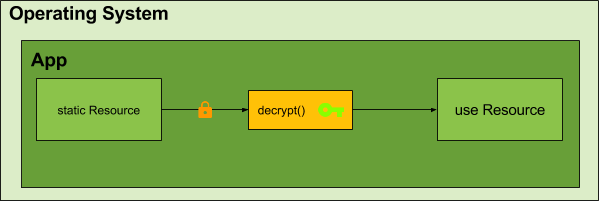
\includegraphics[width=0.8\textwidth]{data/encryptionResource.png}
    \caption{Encrypted resources have to be decrypted before they are used or displayed}
    \label{fig:encryptionResource}
\end{figure}

\subsubsection{Encryption - Action Obfuscator} \label{subsubsectionection:counter-replace-encryption-content-obfuscator}
The second approach is to use encryption a a form of obfuscation.
The idea is to have a single method to delegate all other method calls according to an encrypted parameter.
\newline
When an attacker does a static analysis of the code, the links between method call and executing method are not apparent.
It forces the attacker to use a dynamic analysis method instead.
The fortification of the mechanism is improved when encrypted arguments are passed as well and the decryption is done in the executing method.
This requires more than just opcodes to be circumvented.
\newline
An abstract presentation of the mechanism can be seen in figure~\ref{fig:encryptionAction}.
\begin{figure}[h]
    \centering
    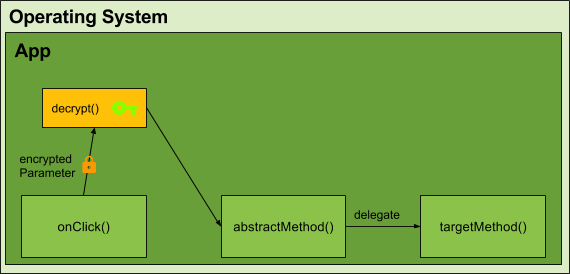
\includegraphics[width=0.8\textwidth]{data/encryptionAction.png}
    \caption{Encrypted actions to obfuscate dependencies}
    \label{fig:encryptionAction}
\end{figure}

\subsubsection{Encryption - Communication} \label{section:counter-replace-encryption-content-communication}
The third approach is to use encryption on the server response as seen in figure~\ref{fig:encryptionComm}.
This additional security feature is applied in combination with a content server as described in subsection~\ref{section:counter-replace-server}.
\newline
When the user does the login on the server, additional unique device specific parameters have to be passed as well, e.g. the \textit{ANDROID\_ID}.
On the first login, the server generates a cryptographic key which is used for communication with the user on this specific device.
The corresponding key can either be generated on the device or be shared by the server.
This mechanism allows only authorized users on a specific device to decrypt the communication.
\newline
\begin{figure}[h]
    \centering
    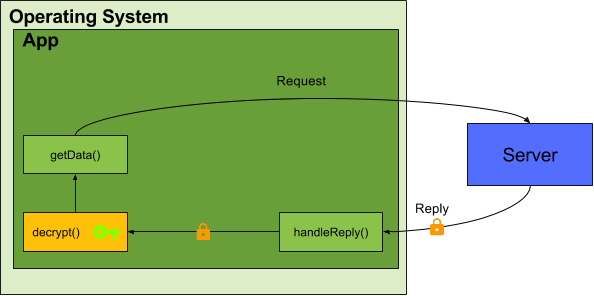
\includegraphics[width=0.8\textwidth]{data/encryptionComm.png}
    \caption{Encrypted communication with a server}
    \label{fig:encryptionComm}
\end{figure}
